\documentclass[12pt, a4paper, twoside]{scrartcl}
 %---- Allgemeine Layout Einstellungen ------------------------------------------

% Für Kopf und Fußzeilen, siehe auch KOMA-Skript Doku
\usepackage[komastyle]{scrpage2}
\pagestyle{scrheadings}
\setheadsepline{0.5pt}[\color{black}]


%Einstellungen für Figuren- und Tabellenbeschriftungen
\setkomafont{captionlabel}{\sffamily\bfseries}
\setcapindent{0em}


%---- Weitere Pakete -----------------------------------------------------------
% Die Pakete sind alle in der TeX Live Distribution enthalten. Wichtige Adressen
% www.ctan.org, www.dante.de

% Sprachunterstützung
\usepackage[ngerman]{babel}

% Benutzung von Umlauten direkt im Text
% entweder "latin1" oder "utf8"
\usepackage[utf8]{inputenc}

% Pakete mit Mathesymbolen und zur Beseitigung von Schwächen der Mathe-Umgebung
\usepackage{latexsym,exscale,stmaryrd,amssymb,amsmath}

% Weitere Symbole
\usepackage[nointegrals]{wasysym}
\usepackage{eurosym}

% Anderes Literaturverzeichnisformat
%\usepackage[square,sort&compress]{natbib}

% Für Farbe
\usepackage{color}

% Zur Graphikausgabe
%Beipiel: \includegraphics[width=\textwidth]{grafik.png}
\usepackage{graphicx}

% Text umfließt Graphiken und Tabellen
% Beispiel:
% \begin{wrapfigure}[Zeilenanzahl]{"l" oder "r"}{breite}
%   \centering
%   \includegraphics[width=...]{grafik}
%   \caption{Beschriftung} 
%   \label{fig:grafik}
% \end{wrapfigure}
\usepackage{wrapfig}

% Mehrere Abbildungen nebeneinander
% Beispiel:
% \begin{figure}[htb]
%   \centering
%   \subfigure[Beschriftung 1\label{fig:label1}]
%   {\includegraphics[width=0.49\textwidth]{grafik1}}
%   \hfill
%   \subfigure[Beschriftung 2\label{fig:label2}]
%   {\includegraphics[width=0.49\textwidth]{grafik2}}
%   \caption{Beschriftung allgemein}
%   \label{fig:label-gesamt}
% \end{figure}
\usepackage{subfigure}

% Caption neben Abbildung
% Beispiel:
% \sidecaptionvpos{figure}{"c" oder "t" oder "b"}
% \begin{SCfigure}[rel. Breite (normalerweise = 1)][hbt]
%   \centering
%   \includegraphics[width=0.5\textwidth]{grafik.png}
%   \caption{Beschreibung}
%   \label{fig:}
% \end{SCfigure}
\usepackage{sidecap}
\usepackage{float}

% Befehl für "Entspricht"-Zeichen
\newcommand{\corresponds}{\ensuremath{\mathrel{\widehat{=}}}}
\newcommand{\folgt}{\ensuremath{\mathrel{\Rightarrow}}}
\newcommand{\equals}{\ensuremath{\mathrel{\Leftrightarrow}}}
\newcommand{\degree}{\ensuremath{\mathrel{^{\circ}}}}

\newcommand{\nn}{\nonumber}
\newcommand{\tn}[1]{\textnormal{#1}}
\newcommand{\D}{\ensuremath{\mathrel{\rm d}}}

\newcommand{\const}{\tn{const}}

\newcommand{\meter}{\ensuremath{\mathrel{\tn m}}}
\newcommand{\kilogramm}{\ensuremath{\mathrel{\tn{kg}}}}
\newcommand{\second}{\ensuremath{\mathrel{\tn s}}}
\newcommand{\sekunde}{\second}

\newcommand{\volt}{\ensuremath{\mathrel{\tn V}}}
\newcommand{\pascal}{\ensuremath{\mathrel{\tn{Pa}}}}
\newcommand{\coulomb}{\ensuremath{\mathrel{\tn C}}}
\newcommand{\newton}{\ensuremath{\mathrel{\tn N}}}
\newcommand{\liter}{\ensuremath{\mathrel{\tn l}}}
\newcommand{\celsius}{\ensuremath{\mathrel{\tn C}}}
\newcommand{\fahrenheit}{\ensuremath{\mathrel{\tn F}}}
\newcommand{\joule}{\ensuremath{\mathrel{\tn J}}}
\newcommand{\kelvin}{\ensuremath{\mathrel{\tn K}}}
\newcommand{\mol}{\ensuremath{\mathrel{\tn{mol}}}}
\newcommand{\gramm}{\ensuremath{\mathrel{\tn{g}}}}

\newcommand{\kilo}{\ensuremath{\mathrel{\tn k}}}
\newcommand{\hecto}{\ensuremath{\mathrel{\tn h}}}

\newcommand{\centi}{\ensuremath{\mathrel{ \tn c}}}
\newcommand{\milli}{\ensuremath{\mathrel{ \tn m}}}
\newcommand{\micro}{\ensuremath{\mathrel{ \tn\mu }}}



%\newcommand{}{\ensuremath{\mathrel{  }}}
%\newcommand{}{\ensuremath{\mathrel{  }}}
%\newcommand{}{\ensuremath{\mathrel{  }}}


\newcommand{\person}[1]{\textsc{#1}}

 \begin{document}
 %Titelseite
\begin{titlepage}
\centering
\textsc{\Large Anfängerpraktikum der Fakultät für
  Physik,\\[1.5ex] Universität Göttingen}

\vspace*{4.2cm}

\rule{\textwidth}{1pt}\\[0.5cm]
{\huge \bfseries
  Spezifische Wärme der Luft und Gasthermometer}\\[0.5cm]
\rule{\textwidth}{1pt}

\vspace*{3.5cm}

\begin{Large}
\begin{tabular}{ll}
Praktikanten: &  Silke Andrea Teepe\\
& Marcel Kramer\\
E-Mail: & \\
Betreuer: & Alexander Schmelev\\
\end{tabular}
\end{Large}

\vspace*{0.8cm}

\begin{Large}
\fbox{
  \begin{minipage}[t][2.5cm][t]{6cm} 
    Testat:
  \end{minipage}
}
\end{Large}

\end{titlepage}
\cleardoublepage
\tableofcontents
\cleardoublepage
\setcounter{page}{1}

\section{Einleitung}


\section{Theorie}
\label{sec:theorie}


\section{Durchführung}
\label{sec:durchfuehrung}

Zur Messung des Dampfdrucks von Wasser ist ein abgeschlossener Kolben zum Teil mit Wasser gefüllt. Dieser Kolben ist auf einer Heizplatte platziert, wodurch dieser erhitzt werden kann. Die Temperatur kann an dem angeschlossenen Pt1000 Widerstandsthermometer abgelesen werden. Der Druck an einem verbundenen Manometer. Aufgrund der hohen Temperatur die während des Experiments erreicht wird gehört aus Sicherheitsgründen auch eine Plexiglas-Schutzscheibe zum Versuchsaufbau. Der beschriebene Aufbau ist auch in Abbildung \ref{img:aufbau} zu sehen.\\


Ziel des Experimentes ist es, die Temperatur in Abhängigkeit des Drucks zu messen. Dazu schaltet man zunächst die Heizplatte ein und notiert dann die entsprechenden Werte von den beiden Messgeräten. Es empfiehlt sich dabei eine Skaleneinteilung von 1-2 bar zu wählen. Sobald entweder $45$ bar oder $1900\,\Omega$ $(240\degree\celsius)$ erreicht sind ist die Heizplatte auszuschalten und die Messung für das Abkühlen zu wiederholen.

\begin{figure} [h]
\centering
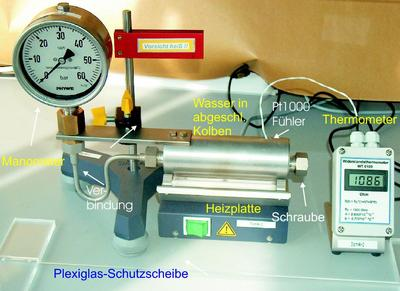
\includegraphics[scale=0.8]{aufbau.jpg}
\caption{\label{img:aufbau}Aufbau des Experiments\protect\footnotemark}
\end{figure}
\footnotetext{https://lp.uni-goettingen.de/get/text/3644}



\section{Auswertung}
\label{sec:auswertung}

\section{Diskussion}
\label{sec:diskussion}

\section*{Literatur}


\end{document}
